\documentclass[a4paper]{article}
\usepackage{tikz}
\usetikzlibrary{decorations}
\usetikzlibrary{decorations.pathmorphing, arrows.meta}
\usetikzlibrary{calc}
\usepackage{apacite}
\usepackage{tabularx}
\usepackage{siunitx}
\usepackage{amsmath}
\usepackage{rotating}
\usepackage{colortbl}
\usepackage{multirow}
\usepackage{arydshln} % Dashed hline
\usepackage{makecell} % Makecell
\usepackage{graphicx}
\usepackage{caption}
\usepackage{footnote}
\usepackage{footmisc}
\usepackage[absolute]{textpos}

% No more than 3000 words.

\renewcommand{\thefootnote}{\roman{footnote}}


\begin{document}


\begin{titlepage}
    \title{\textbf{How does the moment of inertia affect the period of Maxwell's Wheel? \\ \small Physics HL Internal Assessment}}
    \author{mhz237}
    \date{}
    \maketitle
    \centering
    Word count: 2193
    %\tableofcontents
\end{titlepage}

\section{Introduction and background knowledge}

In ancient Greece (around 220 B.C.), Archimedes laid a solid foundation for rigid body statics by discovering and formalizing the conditions of equilibrium for levers. People studied Archimedes's work and developed concepts like torque thereafter, but it was not until Isaac Newton (1643-1727) formulated Laws of Motion that physics became well equipped for rigid body dynamics \cite{farber-1961}. With the assistance of advanced mathematical tools, Leonhard Euler (1707-1783) formalized the dynamics of rigid bodies and derived the concepts of moment of inertia and principal axes \cite{marquina2016leonhard}.

Just like inertia (which is determined by mass) in translational motion, the moment of inertia evaluates a body's ability to resist angular acceleration. Generally speaking, the further away the mass is distributed from its axis of rotation, the larger the body's moment of inertia is. Objects with large moment of inertia are good at storing rotational kinetic energy, which makes them suitable for objects like flywheels, whereas those with small moment of inertia can rotate more rapidly. 

Maxwell's wheel is commonly used as an instrument to illustrate the conservation of energy and the concept of rotational kinetic energy in physics education \cite{pecori1998maxwell}. It can also be utilized to measure the moment of inertia of a disk-shaped object and even the rolling friction if placed on a soft surface \cite{chakrabarti2020}. 

This experiment aims at investigating the significance of the moment of inertia in a Maxwell's wheel experiment. This can help us better understand the rule behind the device and evaluate the pros and cons of Maxwell's Wheel in illustrating physics concepts and principles.

\textbf{Research question: How does the moment of inertia affect the period of Maxwell's Wheel?}

\section{Hypothesis and reasoning}
\label{sec.hypothesis}

\begin{figure}[ht]
    \centering
    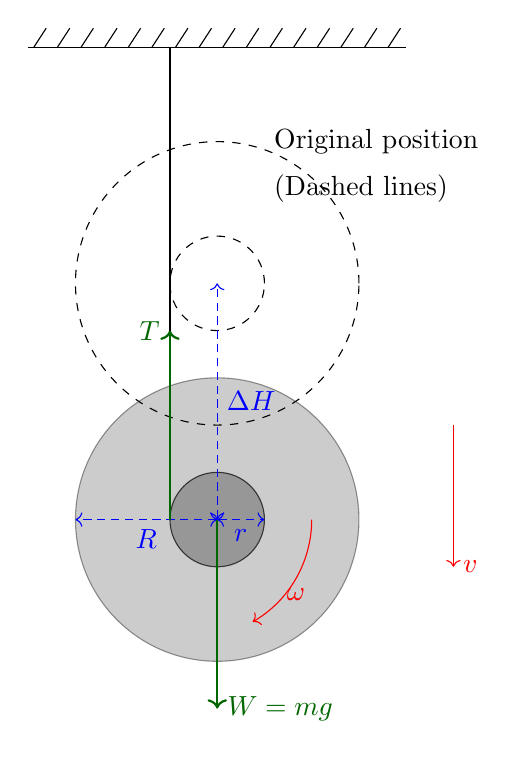
\begin{tikzpicture}[scale = 0.6] % Energy analysis tikzpic 
        \coordinate (O) at (0, 0);
        \draw[fill = gray, opacity = 0.4] (O) circle (3);
        \draw[fill = gray, opacity = 0.7] (O) circle (1);
        \draw[dashed] (0, 5) circle (3);
        \draw[dashed] (0, 5) circle (1);
        \node[right] at (1, 8) {Original position};
        \node[right] at (1, 7) {(Dashed lines)};
        \draw (-4, 10) -- (4, 10);
        \foreach \x in {-3.75, -3.25, ..., 3.75} 
            \draw[xshift = \x cm] (0.13, 10.4) -- (-0.13, 10);
        \draw[thick] (-1, 4) -- (-1, 10); 

        % Lengths
        \draw[<->, densely dashed, blue] (0, 0) -- (1, 0) node[midway, below, scale = 1] {$r$};
        \draw[<->, densely dashed, blue] (0, 0) -- (-3, 0) node[midway, below, scale = 1] {$R$};
        \draw[<->, densely dashed, blue] (0, 0) -- (0, 5) node[midway, right, scale = 1] {$\Delta H$};

        % Kinetics
        \draw[->, red] (5, 2) -- (5, -1) node[right, scale = 1] {$v$};
        \draw[->, red] (2, 0) arc (0: -60: 2.5) node[midway, right, below, scale = 1] {$\omega$};

        % Forces
        \draw[->, black!60!green, thick] (-1, 0) -- (-1, 4) node[above, left, scale = 1] {$T$};
        \draw[->, black!60!green, thick] (0, 0) -- (0, -4) node[below, right, scale = 1] {$W = mg$};
    \end{tikzpicture}
    \caption{Model of a Maxwell's Wheel}
    \label{fig.maxwellwheel}
\end{figure}

As is shown in Figure \ref{fig.maxwellwheel}, the Maxwell's wheel mainly consists of three parts: a disk-shaped wheel of radius $R$, an axle of radius $r$ penetrating the wheel, and a string that swirls around the axle. Aside from friction, two forces are acting on the pendulum: the upward tension from the string and the gravitational force downward. During the entire process, the gravitational potential energy converts to kinetic energy of the wheel. 

The downward movement and the upward movement are approximately symmetric, so only the downward process needs algebraic analysis.

Since the wheel is not in equilibrium, its challenging to analyze the magnitude of tension $T$. However, the problem can be appraached using conservation of energy.

Neglecting friction, it can be assumed that all the gravitational potential energy lost is converted to the kinetic energy. Or more specificaly, the sum of the translational kinetic energy and rotational kinetic energy should equal to the loss in gravitational potential energy, as is formally stated in Equation \ref{eq.con}.

\begin{equation}\label{eq.con}
    mg\Delta h = \frac{1}{2}m v^2 + \frac{1}{2} I \omega ^2
\end{equation}
% IDK, maybe the original version is better? 

where $I$ is the moment of inertia of the entire wheel. 

Moreover, using the definition of velocity and angular velocity, we can derive identities \ref{eq.defv}, \ref{eq.defomega}, and \ref{eq.h0}.

\begin{equation}\label{eq.defv}
    \dfrac{\mathrm{d}\Delta H}{\mathrm{d}t} = v
\end{equation}

\begin{equation}\label{eq.defomega}
    \omega r = v
\end{equation}

\begin{equation}\label{eq.h0}
    \Delta H(0) = 0
\end{equation}

Therefore, after replacing $\omega$ in Equation \ref{eq.con} with Equation \ref{eq.defomega}, we can get Equation \ref{eq.general}, whose terms can be moved and combined and $v$ can be replaced using Equation \ref{eq.defv} to derive Equation \ref{eq.separate}.

\begin{equation}\label{eq.general}
    mg\Delta H = \frac{1}{2}m v^2 + \frac{1}{2} \frac{I}{r^2} v ^2
\end{equation}

\begin{equation}\label{eq.separate}
    \frac{2mg\Delta H}{m+\frac{I}{r^2}} = (\dfrac{\mathrm{d}\Delta H}{\mathrm{d}t})^2
\end{equation}

Moving ${\mathrm{d}\Delta H}/{\mathrm{d}t}$ to the left side and make its index $1$, a simple ODE (Ordinary Differential Equation) for $\Delta H(t)$ is obtained, as is shown in Equation \ref{eq.odeform}.

\begin{equation}\label{eq.odeform}
    \dfrac{\mathrm{d}\Delta H}{\mathrm{d}t} = \sqrt{\frac{2mg}{m+\frac{I}{r^2}}} \Delta H ^ {0.5}
\end{equation}

By letting coefficient $k$ be $\sqrt{\frac{2mg}{m+\frac{I}{r^2}}}$, the ODE can be solved by separating variables and integrating the both sides, as is shown in Equation \ref{eq.solveode}.

\begin{equation}
    \label{eq.solveode}
    \begin{aligned}
        \dfrac{\mathrm{d}\Delta H}{\mathrm{d}t} &= k \Delta H ^ {0.5}\\
        \Delta H ^ {-0.5} \mathrm{d}\Delta H  &= k\mathrm{d}t \\
        \int \Delta H ^ {-0.5} \mathrm{d}\Delta H &= \int k\mathrm{d}t \\
        2\Delta H ^ {0.5} &= k t + C\\
    \end{aligned}
\end{equation}

With the help of initial condition Equation \ref{eq.h0}, we know that $C = 0$. 

\begin{equation}
    \begin{aligned}
        2\Delta H ^ {0.5} &= k t \\
        \Delta H  &= (\dfrac{k}{2})^2 t^2 \\
    \end{aligned}
\end{equation}

Therefore the ODE is solved, and the solution is Equation \ref{eq.h}.

\begin{equation}\label{eq.h}
    \Delta H(t) = \dfrac{k^2}{4} t^2 = \dfrac{mg}{2m+\frac{2I}{r^2}} t^2
\end{equation}

The downward movement terminates when $\Delta H(t) = l$, where $l$ is the length of the string. Therefore, the time for downward movement $t_{down}$ is calculated as Equation \ref{eq.tdown}.

\begin{equation}\label{eq.tdown}
    \begin{aligned}
        \Delta H(t_{down}) = \dfrac{k^2}{4} t_{down}^2 &= l\\
        t_{down} &= 2\sqrt{\dfrac{l}{k^2}}
    \end{aligned}
\end{equation}

Since the downward and upward movements are symmetric, the entire period of the Maxwell's Wheel can be formulated in Equation \ref{eq.period}.

\begin{equation}\label{eq.period}
    T = 2t_{down} = 4\sqrt{\dfrac{l}{k^2}}
\end{equation}

When both sides are squared, we can get Equation \ref{eq.t2}, which can be further simplified by separating terms with and without $I$ to get Equation \ref{eq.t22}.

\begin{equation}\label{eq.t2}
    T^2 = 16\dfrac{l}{k^2} = 8l\dfrac{(m+\frac{I}{r^2})}{mg}
\end{equation}

\begin{equation}\label{eq.t22}
    T^2 = \dfrac{8l}{mgr^2} I + \dfrac{8l}{g}
\end{equation}

From this formula, the hypothesis can be derived: \textbf{$T$ increases as $I$ increases. $T^2$ and $I$ has a linear relationship.} When $T^2$ is plotted against $I$, a straight line with a positive gradient and positive y-intercept is expected.

\section{Experiment design}

\subsection{Variables} 

\begin{itemize}
    \item Independent variable: Moment of inertia (manipulated by changing the distance from the magnets to the pivot: $r' = \SI{2.5}{cm}, \SI{3.5}{cm}, \SI{4.5}{cm}, \SI{5.5}{cm},\allowbreak \SI{6.5}{cm}, \SI{7.5}{cm}, \SI{8.5}{cm}$).
    \item Dependent variable: ``Period'' of the Maxwell's Wheel (Time between two lowest positions).
    \item Controlled variables: The material, mass and size of the plate and magnets. The length of the string. The mass, radius and length of the axle, etc. They are listed in Table \ref{tab.control}.
\end{itemize}

%Controlled variable table:

\begin{table}[ht!]
\centering
\caption{Controlled variables}
\label{tab.control}
\begin{tabularx}{\textwidth}{p{2.0cm}p{1.5cm}XX}
\hline
Variable                    & Value                  & Reason to control                                          & Method to control                                    \\ \hline
Total mass of the wheel $m$ & $\approx \SI{400}{g}$  & To ensure the gradient is not affected.                 & Use the same set of magnets, plate and axle.         \\
Material of the wheel       & Acrylic + NdFeB magnet & To ensure the mass distribution is even and consistent. & Use the same set of magnets and plate.               \\
Height of displacement      & $\approx \SI{20}{cm}$  & Unify the initial kinetic energy and length of path.       & Determine and mark a release position on the string. \\ 
Temperature and humidity    & Around 25$^\circ$C, 40\% RH  & Avoid the change in air resistance                   & Conduct the experiment in a short period of time.    \\\hline
\end{tabularx}
\end{table}

\subsection{Materials}

\begin{itemize}
    \item[*] 2 Retort stands (height $\approx \SI{50}{cm}$) with clamps
    \item[*] 2 Cotton strings (length $\approx \SI{70}{cm}$)
    \item[*] 1 Acrylic disc with axle (radius $\approx \SI{10}{cm}$, mass $\approx \SI{110}{g}$)
    \item[*] 16 Round magnets (radius $\approx \SI{3.0}{cm}$, mass $\approx \SI{23}{g}$)
    \item[*] 1 Electric force gauge ($\SI{50}{N}$), with compatible data cable
    \item[*] 1 Tape rule (range $\ge \SI{50}{cm}$, resolution $\le \SI{0.1}{cm}$)
    \item[*] 1 Electric balance (range $\ge \SI{400}{g}$, resolution $\le \SI{0.1}{g}$)
    \item[*] 1 Vernier caliper (range $\ge \SI{5}{cm}$, resolution $\le \SI{0.01}{cm}$)
    \item[*] 1 Hot glue gun  
\end{itemize}

\subsection{Setup diagram}

The apparatus is set up by hanging the Maxwell's Wheel between two iron stands using cotton string, as is shown in Figure \ref{fig.setup}.

\begin{figure}[ht]
    \centering
    \includegraphics[width = 0.8\textwidth]{setup.png}
    \caption{Setup diagram $^{2}$}
    \label{fig.setup}
    \begin{minipage}{0.8\textwidth}
    \begin{flushleft}
        \footnotesize{1 The rough location of rolling up is marked with a rubber band and the precise location is marked with a pen.} \\
        \footnotesize{2 The graph is made with chemix and mspaint.}
    \end{flushleft}
    \end{minipage}
    
\end{figure}

\subsection{Procedure}

\begin{enumerate}
    \item Measure the total mass of the magnets, mass of the acrylic plate, radius of the acrylic plate, radius of the axle and maximum vertical displacement after setting up the apparatus as is shown in Figure \ref{fig.setup}
    \item Find a pair of diameters of the acrylic plane that is perpendicular to each other. This can be done by drawing the perpendicular bisector of an arbitrary pair of perpendicular chords. 
    \item Calibrate both axis with the assistance of a ruler. Make sure the center of the circle is scaled zero. 
    \item Attach four pairs of magnets to the plane.
    \item Adjust the position of the magnets to make the distance for the magnets' centers of mass are $r = \SI{8.5}{cm}$. This can be done by placing the magnet (with radius $r' = \SI{3}{cm}$) between $r = \SI{10}{cm}$ mark and $r = \SI{7}{cm}$ mark, while touching the both marks.
    \item Fix the magnets with the glue gun to prevent them from sliding on the plate.
    \item Swirl up the axle until it reaches the designated point, start the forcemeter and release the wheel. 
    \item Record the time for the first and second time where the forcemeter reading reaches local maxima. Take them down as $t_1$ and $t_2$. \footnote{This is done with the assistance of a program. If the first local maximum is not prominant, the second and the third local maxima is used instead.} 
    \item Repeat Steps 7 and 8 for $4$ additional trials.
    \item Repeat Steps 5 to 9 with $r = \SI{7.5}{cm}, \SI{6.5}{cm}, \SI{5.5}{cm}, \SI{4.5}{cm}, \SI{3.5}{cm}$.
\end{enumerate}

\subsection{Risk assessment}

The experiment is relatively safe with little potential hazard. 

It is worth keeping in mind that one should exercise caution when using the magnets, since the strong attraction of the magnets can cause unintended damage to the operator (e.g. their skin may be pinched when the magnets snaps together).

The experiment does not involve ethical issues as no human or animal subjects are involved.

The experiment has little environmental issues as little material is disposed and none of the materials are toxic.

\section{Results}
\label{sec.results}

\subsection{Raw data}

The raw data were collected as follows:

\begin{itemize}
    \item Total mass of the magnets $M_m$ : $179.39\pm0.01\SI{}{g}$
    \item Total mass of the acrylic plate $M_a$: $111.2\pm0.01\SI{}{g}$
    \item Radius of the acrylic plate $R_a$: $10.0\pm0.05\SI{}{cm}$
    \item Radius of the axle $r$: $4.0\pm0.1\SI{}{mm}$
    \item Maximum vertical displacement $H$: $20\pm0.5\SI{}{cm}$
    \item Other data are presented in Table \ref{tab.raw} (where $r'$ denotes the distance from the center of mass of the magnets to the pivot and $t_1$ and $t_2$ represent the times for the first and second local maxima respectively).
\end{itemize}

\begin{table}[ht]
\centering
\caption{Raw Data}
\label{tab.raw}
\begin{tabularx}{\textwidth}{XXXXXXXXXX}
\hline
\hline
\multicolumn{5}{c}{Experiments 1-4} & \multicolumn{5}{c}{Experiments 5-7} \\
\hline
No.         & \makecell{$r'(\SI{}{cm})$ \\ $\pm \SI{0.1}{cm}$ }  & Trial & \makecell{$t_1(\SI{}{s})$ \\ $\pm \SI{0.01}{s}$ } & \makecell{$t_2(\SI{}{s})$ \\ $\pm \SI{0.01}{s}$ } & 
No.         & \makecell{$r'(\SI{}{cm})$ \\ $\pm \SI{0.1}{cm}$ }  & Trial & \makecell{$t_1(\SI{}{s})$ \\ $\pm \SI{0.01}{s}$ } & \makecell{$t_2(\SI{}{s})$ \\ $\pm \SI{0.01}{s}$ } \\
\hline
\multirow{5}{*}{1} & \multirow{5}{*}{$2.5$} & 1     & $2.28$   & $6.68$   & 
\multirow{5}{*}{5} & \multirow{5}{*}{$6.5$} & 1     & $3.58$   & $9.48$   \\
                   &                                & 2     & $2.25$   & $6.63$   &
                   &                                & 2     & $9.28$   & $15.23$  \\
                   &                                & 3     & $2.48$   & $7.03$   &
                   &                                & 3     & $3.45$   & $9.48$   \\
                   &                                & 4     & $6.73$   & $11.28$  &
                   &                                & 4     & $3.53$   & $9.43$   \\
                   &                                & 5     & $2.33$   & $6.78$   &
                   &                                & 5     & $9.28$   & $15.23$   \\
\cdashline{1-5} \cdashline{6-10}
\multirow{5}{*}{2} & \multirow{5}{*}{$3.5$} & 1     & $2.73$   & $7.23$   & 
\multirow{5}{*}{6} & \multirow{5}{*}{$7.5$} & 1     & $10.43$  & $17.68$  \\
                   &                                & 2     & $7.03$   & $11.53$  &
                   &                                & 2     & $3.93$   & $10.68$  \\
                   &                                & 3     & $2.78$   & $7.63$   &
                   &                                & 3     & $4.08$   & $11.03$  \\
                   &                                & 4     & $2.58$   & $7.38$   &
                   &                                & 4     & $4.23$   & $11.13$  \\
                   &                                & 5     & $2.83$   & $7.33$   &
                   &                                & 5     & $4.03$   & $10.53$   \\
\cdashline{1-5} \cdashline{6-10}
\multirow{5}{*}{3} & \multirow{5}{*}{$4.5$} & 1     & $2.88$   & $8.13$   & 
\multirow{6}{*}{7} & \multirow{6}{*}{$8.5$} & 1     & $4.08$   & $11.78$  \\
                   &                                & 2     & $3.18$   & $8.63$   &
                   &                                & 2     & $11.68$  & $18.33$  \\
                   &                                & 3     & $3.08$   & $8.53$   &
                   &                                & 3     & $11.48$  & $18.38$  \\
                   &                                & 4     & $2.88$   & $7.88$   &
                   &                                & 4     & $12.03$  & $20.58$  \\
                   &                                & 5     & $3.03$   & $8.28$   &
                   &                                & 5     & $11.78$  & $18.63$   \\
\cdashline{1-5}
\multirow{5}{*}{4} & \multirow{5}{*}{$5.5$} & 1     & $3.28$   & $8.93$   &
                   &                                & 6     & $4.13$   & $11.63$   \\
\cdashline{6-10}
                   &                                & 2     & $3.23$   & $8.73$   & & & & & \\
                   &                                & 3     & $3.23$   & $8.83$   & & & & & \\
                   &                                & 4     & $3.18$   & $8.73$   & & & & & \\
                   &                                & 5     & $3.48$   & $9.23$   & & & & & \\
%\cdashline{1-5}
\hline
\hline
\end{tabularx}
\end{table}

\newpage

\subsection{Processed data} 

The $I_a$, the moment of inertia due to the plate, is the same ($5.56 \pm 0.112\times10^{-4}\SI{}{kgm^2}$) for each trial, as is given in Section \ref{sec.sample}. Other processed data are listed in Table \ref{tab.proc}, where $I_m$ is the moment of inertia due to magnets, $T$ is the period, $T^2$ is the square of the period. The data is plotted in Figure \ref{fig.processedd}.

% More details should be included.
\label{sec.procd}

\begin{table}[ht]
\centering
\caption{Processed data}
\label{tab.proc}
\begin{tabular}{lllll}
\hline \hline
Exp. &
$ I_m (\times10^{-4}\SI{}{kgm^2}) $ &
$ I_{tot} (\times10^{-3}\SI{}{kgm^2}) $ &
$ \bar{T} (\SI{}{s}) $ &
$ T^2 (\SI{}{s^2}) $ \\ \hline
1 & $1.12 \pm 0.10$ & $0.668 \pm 0.020$ & $4.466 \pm 0.085$ & $19.9 \pm 0.76$ \\
2 & $2.20 \pm 1.26$ & $0.776 \pm 0.024$ & $4.63 \pm 0.18$ & $21.4 \pm 1.62$ \\
3 & $3.63 \pm 1.62$ & $0.919 \pm 0.053$ & $5.28 \pm 0.23$ & $27.9 \pm 2.38$ \\
4 & $5.43 \pm 1.98$ & $1.099 \pm 0.031$ & $5.61 \pm 0.13$ & $31.5 \pm 1.40$ \\
5 & $7.58 \pm 2.34$ & $1.314 \pm 0.035$ & $5.946 \pm 0.065$ & $35.4 \pm 0.77$ \\
6 & $10.09 \pm 2.70$ & $1.566 \pm 0.038$ & $6.87 \pm 0.38$ & $47.2 \pm 5.15$ \\
7 & $12.96 \pm 3.06$ & $1.852 \pm 0.042$ & $7.12 \pm 0.53$ & $50.7 \pm 7.48$ \\ \hline \hline
\end{tabular}
\end{table}


\begin{figure}[ht]
    \centering
    \includegraphics[width = 0.8\textwidth]{grapha.png}
    \caption{$T^2 - I$ graph}
    \label{fig.processedd}
\end{figure}

\subsection{Sample processing}

\label{sec.sample}

Take the data processing of experiment $1$ as an example. 

The $R$, distance from the magnets' center of mass to the pivot, is measured to be $2.5\pm 0.1\SI{}{cm}$. Therefore the moment of inertia contributed by the magnets is calculated as Equations \ref{eq.imagnet} and \ref{eq.dimagnet}.

\begin{equation}
    \begin{aligned}
        I_m &= M_m \times r'^2 \\
            &= 179.39 \times 10^{-3} \SI{}{kg} \times( 2.5 \times 10^{-2})^2 \SI{}{m^2}\\
            &= 1.1\times 10^{-4}\SI{}{kgm^2}
    \end{aligned}
    \label{eq.imagnet}
\end{equation}% 1.112119

\begin{equation}
    \begin{aligned}
        \Delta I_m &= \%\Delta I_m \times I_m \\
            &= (\frac{\Delta M}{M} + 2\frac{\Delta R}{R})\times I_m\\
            &= \pm 9\times 10^{-6}\SI{}{kgm^2}
    \end{aligned} 
    \label{eq.dimagnet}
\end{equation}

Furthermore, the moment of inertia contributed by the acrylic disk is calculated as in Equations \ref{eq.idisk} and \ref{eq.didisk}.

\begin{equation}
    \begin{aligned}
        I_a &= \dfrac{1}{2}M_a \times R_a^2 \\
            &= 111.2 \times 10^{-3} \SI{}{kg} \times( 10.0 \times 10^{-2})^2 \SI{}{m^2}\\
            &= 5.56\times 10^{-4}\SI{}{kgm^2}
    \end{aligned}
    \label{eq.idisk}
\end{equation}

\begin{equation}
    \begin{aligned}
        \Delta I_a &= \%\Delta I_a \times I_a \\
            &= (\frac{\Delta M}{M} + 2\frac{\Delta R}{R})\times I_a\\
            &= \pm 1.12\times 10^{-5}\SI{}{kgm^2}
    \end{aligned} 
    \label{eq.didisk}
\end{equation}

The total moment of inertia $I$ is calculated as in Equation \ref{eq.i} and the uncertainty is calculated as in Equation \ref{eq.di}.

\begin{equation}
    \begin{aligned}
        I &= I_m + I_a \\
            &= 1.1\times 10^{-4}\SI{}{kgm^2} + 5.56\times 10^{-4}\SI{}{kgm^2}\\
            &= 6.68\times 10^{-4}\SI{}{kgm^2}
    \end{aligned}
    \label{eq.i}
\end{equation}

\begin{equation}
    \begin{aligned}
        \Delta I &= \Delta I_m + \Delta I_a\\
                 &= \pm(9\times 10^{-6}\SI{}{kgm^2} + 1.12\times 10^{-5}\SI{}{kgm^2})\\
                 &= \pm 2.02\times 10^{-5}\SI{}{kgm^2}
    \end{aligned}
    \label{eq.di}
\end{equation}

The force gauge data is recorded and plotted against time in Figure \ref{fig.ft}. It can be noticed that the reading of the force gauge is noisy but shows clear peaks. With the assistance of a program, prominent peaks are marked in the figure using red dots.

\begin{figure}[ht]
    \centering
    \includegraphics[width = \textwidth]{graphft.png}
    \caption{$F - t$ graph sample}
    \label{fig.ft}
\end{figure}

The x-index of the first two peaks are taken as $t_1$ and $t_2$ of this trial. The ``period" of the experiment $T_a$ is calculated as in Equation \ref{eq.ta}, whose uncertainty is calculated as in Equation \ref{eq.dta}.

\begin{equation}
    \begin{aligned}
        T_a &= t_1 - t_0 \\
            &= \SI{6.68}{s} -  \SI{2.28}{s}\\
            &= \SI{4.40}{s}
    \end{aligned}
    \label{eq.ta}
\end{equation}

\begin{equation}
    \begin{aligned}
        \Delta T_a &= \Delta t_1 + \Delta t_0 \\
                   &= (\pm \SI{0.01}{s}) + (\pm\SI{0.01}{s}) \\
                   &= \pm \SI{0.02}{s}
    \end{aligned}
    \label{eq.dta}
\end{equation}

Applying this to five trials, we can get the average of the first experiment and the corresponding uncertainties, as is shown in Equations \ref{eq.tavg} and \ref{eq.dtavg}.

\begin{equation}
    \begin{aligned}
        \overline{T} &= \frac{T_a + T_b + T_c + T_d + T_e}{5} \\
                &= \SI{4.466}{s}
    \end{aligned}
    \label{eq.tavg}
\end{equation}

\begin{equation}
    \begin{aligned}
        \Delta\overline{T} &= \frac{\max\{T_i\} - \min\{T_i\}}{2} \\
                      &= \frac{\SI{4.55}{s} - \SI{4.38}{s}}{2} \\
                      &= \SI{0.085}{s}
    \end{aligned}
    \label{eq.dtavg}
\end{equation}

Therefore the square of the period can be calculated as in Equations \ref{eq.t2avg} and \ref{eq.dt2avg}.

\begin{equation}
    \begin{aligned}
        \overline{T}^2 &= (\SI{4.466}{s})^2\\
                        &= \SI{19.94}{s^2}
    \end{aligned}
    \label{eq.t2avg}
\end{equation}

\begin{equation}
    \begin{aligned}
        \Delta\overline{T}^2 &= \frac{\Delta\overline{T}}{\overline{T}}\times 2 \times \overline{T}^2\\
                        &= 1.9032\% \times 2 \times \SI{19.94}{s^2}\\
                        &= \SI{0.7592}{s^2}
    \end{aligned}
    \label{eq.dt2avg}
\end{equation}


\section{Discussion and conclusion}

% Direct observation from tables.

\label{sec.discussion}

The diagram Figure \ref{fig.processedd} indicates strong correlation between $T^2$ and $I$. The best fit line of $T^2 - I$ has 
% directly describe the graph

\begin{itemize}
    \item a gradient of $(27.3150 \pm 6.9556) \times 10^3\ \SI{}{s^2kg^{-1}m^{-2}}$.
    \item a y-intercept of $1.4557 \SI{}{s^2}$ \footnote{The uncertainty is meaningless as the increasing uncertainty of $T^2$ results in exaggerated uncertainty of the y-intercept}. 
\end{itemize}

% Notes:
% Correlation coefficient should be discussed. 
% local gravity acceleration (?)

As is mentioned in Section \ref{sec.hypothesis}, the graph is expected to be a straight line very close to the origin. The diagram presents a graph with relatively small error, supporting the initial hypothesis.

The y-intercept is expected to be $\frac{8l}{mgr^2} \approx 0.16\SI{}{s^2}$, but $1.4557\SI{}{s^2}$ is found. This is almost $9$ times the theoretical value. However, considering the large value of $T$ in the dataset, $1.4557\SI{}{s^2}$ is still less than $10\%$ of the minimum dependent variable. This means it can still be considered an error, whose cause will be discussed in Section \ref{sec.eval}.

\begin{equation}
    \label{eq.deltapk}
    \Delta\% k = \frac{|k - k_0|}{k} \times 100\% = \frac{27.3150 - 26.3900}{26.3900} \times 100\% = 3.51\%
\end{equation}

The gradient is expected to be $\frac{8l}{g} = 26.3900 \times 10^3\ \SI{}{s^2kg^{-1}m^{-2}}$, where $l$ is the length for lifting (controlled to be close to $\SI{20}{cm}$) and $g$ is the gravitational acceleration near sea level. There is a small $3.51\%$ error (as is shown in Equation \ref{eq.deltapk}) between the actual gradient and predicted gradient, and the predicted gradient lies within the uncertainty range of the gradient. The low error indicates high accuracy and precision of this experiment.

Horizontal error bars are too small to be displayed in the graph, showing high precision and accuracy when manipulating the independent variable. Vertical error bars are small when $I$ is small, but becomes larger as $I$ gets larger. That might result from the significant horizontal perturbation getting greater as $I$ increases. Horizontal movements causes the wheel start to swing like a pendulum and makes the motion more chaotic and less trackable. 

The best fit line fails to pass through the fifth error bar, which is also coincidentally a very small error bar. That might be due to coincidence, since there are only five trials in each group.

Therefore, we can conclude that the period increases as the moment of inertia increases. The square of the period and the moment of inertia has a linear relationship.

\section{Evaluation}
\label{sec.eval}

The experiment was conducted successfully, gathering sufficient data and supporting the initial hypothesis. The graphs are similar to the graphs in Pecori et al.'s \citeyear{pecori1998maxwell} and Gianino et al.'s \citeyear{gianino2024analysis} experiments with similar conclusions. However, there are some parts in the experiment that can be improved. 

\begin{itemize}
    \item \textbf{Defect in modelling} It is assumed in the hypothesis that the wheel does not swing horizontally and the string is always vertical, but small horizontal movement is inevitable during the experiment, as the extended line of the string does not go through the wheel's center of mass. Using a plumb line to adjust the string before releasing can minimize the horizontal deflection. A more advanced model taking that into consideration can provide a more precise prediction.
    \item \textbf{Energy loss} The model negelected the effect of air resistance and other form of energy loss during the process, which means the energy during the experiment is lower than expected. Considering the damping in the model can make the model more accurate.
    \item \textbf{Screw-threaded axle} For an ideal Maxwell's Wheel, the radius of the small axle should be constant. However, a screw-threaded axle is utilized to ensure better installation of the wheel, making the string swirl around the thread with inconsistent radius. This can be improved by using an axle that has screw thread only in the middle point. 
    \item \textbf{String attaching} When attaching the wire to the axle, some adhesive (hot glue) is used to ensure connection stability. This also contributed to inconsistent radius. An axle with a hole for attachment can eliminate the need for adhesive.
    \item \textbf{Imprecise marking on the string} The string is not vertical to the ground, which means the marked distance is not precisely the vertical displacement. Additionally, axle's size can also lead to inconsistant vertical displacement. This might have lead to unexpected large y-intercept mentioned in Section \ref{sec.discussion}. Using a plumbline to ensure perpendicularity can result in better measurement.
    \item \textbf{Stretching of the string} When the Maxwell's Wheel reaches the lowermost position, the downward movement is changed to an upward one with approximately same magnitude. However, as \cite{pecori1998maxwell} suggests, this happnes because of the stretching of the string. Such process took about $\SI{0.16}{s}$ in Percori's experiment but it could not be measured accurately in the experiment due to different string material and the machine's sampling frequency. This can lead to longer ``period'' than expected, and can be compensated using a forcemeter with faster sampling speed.  
    \item \textbf{Method of independent variable manipulation}  The independent variable is hard to manipulate, as the moment of inertia results from the arithmetical addition of two parts: the acrylic disk and the magnets. The former part is independent of $r'$, making it impossible to reach very small $I$. The latter part is proportional to $r'^2$, resulting in difficulty to place the magnets on the acrylic plane if even distribution between $I$ is needed. Lighter disk with larger size can make the manipulation easier.
    \item \textbf{Local gravitational acceleration} The gravitational acceleration is dependent on the region and is not always consistent with the $g$ taken. This can result in deviated hypothesis and can be improved by looking up local gravitational acceleration online.
    \item \textbf{Only 7 groups of data and 5 trials for each group} Limited number of trials make the result not convincing enough. It would be better if more independent variables are chosen and more trials are conducted.
\end{itemize}

\bibliographystyle{apacite}
\bibliography{cit.bib}

\end{document}